%\input{Preambulum}

\begin{figure}[t!]
\centering
\begin{subfigure}{0.24\textwidth}
\centering
\caption{$H_1$: $0 / 24$}
\label{Fig2_1}

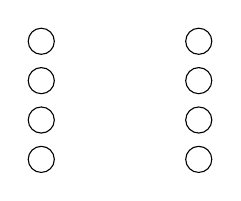
\begin{tikzpicture}[scale=1, auto=center]
\tikzstyle{every node}=[draw,shape=circle];
  \node[minimum size=0.25cm] (n1) at (0,1.5) {};
  \node[minimum size=0.25cm] (n2) at (0,1) {};
  \node[minimum size=0.25cm] (n3) at (0,0.5) {};
  \node[minimum size=0.25cm] (n4) at (0,0) {};
  \node[minimum size=0.25cm] (n5) at (2,1.5) {};
  \node[minimum size=0.25cm] (n6) at (2,1) {};
  \node[minimum size=0.25cm] (n7) at (2,0.5) {};
  \node[minimum size=0.25cm] (n8) at (2,0) {};

  \foreach \from/\to in {}
    \draw (\from) -- (\to);
\end{tikzpicture}
\end{subfigure}
\begin{subfigure}{0.24\textwidth}
\centering
\caption{$H_2$: $1 / 18$}
\label{Fig2_2}

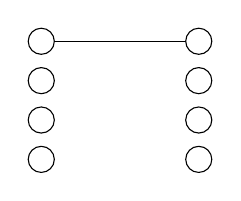
\begin{tikzpicture}[scale=1, auto=center]
\tikzstyle{every node}=[draw,shape=circle];
  \node[minimum size=0.25cm] (n1) at (0,1.5) {};
  \node[minimum size=0.25cm] (n2) at (0,1) {};
  \node[minimum size=0.25cm] (n3) at (0,0.5) {};
  \node[minimum size=0.25cm] (n4) at (0,0) {};
  \node[minimum size=0.25cm] (n5) at (2,1.5) {};
  \node[minimum size=0.25cm] (n6) at (2,1) {};
  \node[minimum size=0.25cm] (n7) at (2,0.5) {};
  \node[minimum size=0.25cm] (n8) at (2,0) {};

  \foreach \from/\to in {n1/n5}
    \draw (\from) -- (\to);
\end{tikzpicture}
\end{subfigure}
\begin{subfigure}{0.24\textwidth}
\centering
\caption{$H_{3-5}$: $2 / 14$}
\label{Fig2_3}

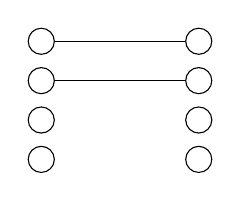
\begin{tikzpicture}[scale=1, auto=center]
\tikzstyle{every node}=[draw,shape=circle];
  \node[minimum size=0.25cm] (n1) at (0,1.5) {};
  \node[minimum size=0.25cm] (n2) at (0,1) {};
  \node[minimum size=0.25cm] (n3) at (0,0.5) {};
  \node[minimum size=0.25cm] (n4) at (0,0) {};
  \node[minimum size=0.25cm] (n5) at (2,1.5) {};
  \node[minimum size=0.25cm] (n6) at (2,1) {};
  \node[minimum size=0.25cm] (n7) at (2,0.5) {};
  \node[minimum size=0.25cm] (n8) at (2,0) {};

  \foreach \from/\to in {n1/n5,n2/n6}
    \draw (\from) -- (\to);
\end{tikzpicture}
\end{subfigure}
\begin{subfigure}{0.24\textwidth}
\centering
\caption{$H_{6-8}$: $3 / 11$}
\label{Fig2_4}

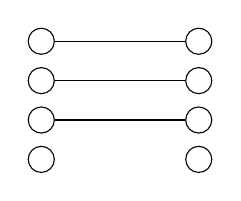
\begin{tikzpicture}[scale=1, auto=center]
\tikzstyle{every node}=[draw,shape=circle];
  \node[minimum size=0.25cm] (n1) at (0,1.5) {};
  \node[minimum size=0.25cm] (n2) at (0,1) {};
  \node[minimum size=0.25cm] (n3) at (0,0.5) {};
  \node[minimum size=0.25cm] (n4) at (0,0) {};
  \node[minimum size=0.25cm] (n5) at (2,1.5) {};
  \node[minimum size=0.25cm] (n6) at (2,1) {};
  \node[minimum size=0.25cm] (n7) at (2,0.5) {};
  \node[minimum size=0.25cm] (n8) at (2,0) {};

  \foreach \from/\to in {n1/n5,n2/n6,n3/n7}
    \draw (\from) -- (\to);
\end{tikzpicture}
\end{subfigure}

%\vspace{0.25cm}
\begin{subfigure}{0.24\textwidth}
\centering
\caption{$H_{9-10}$: $4 / 9$}
\label{Fig2_5}

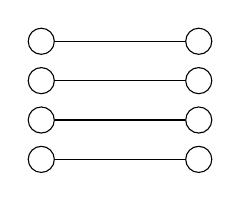
\begin{tikzpicture}[scale=1, auto=center]
\tikzstyle{every node}=[draw,shape=circle];
  \node[minimum size=0.25cm] (n1) at (0,1.5) {};
  \node[minimum size=0.25cm] (n2) at (0,1) {};
  \node[minimum size=0.25cm] (n3) at (0,0.5) {};
  \node[minimum size=0.25cm] (n4) at (0,0) {};
  \node[minimum size=0.25cm] (n5) at (2,1.5) {};
  \node[minimum size=0.25cm] (n6) at (2,1) {};
  \node[minimum size=0.25cm] (n7) at (2,0.5) {};
  \node[minimum size=0.25cm] (n8) at (2,0) {};

  \foreach \from/\to in {n1/n5,n2/n6,n3/n7,n4/n8}
    \draw (\from) -- (\to);
\end{tikzpicture}
\end{subfigure}
\begin{subfigure}{0.24\textwidth}
\centering
\caption{$H_{11}$: $2 / 12$}
\label{Fig2_6}

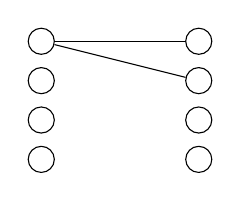
\begin{tikzpicture}[scale=1, auto=center]
\tikzstyle{every node}=[draw,shape=circle];
  \node[minimum size=0.25cm] (n1) at (0,1.5) {};
  \node[minimum size=0.25cm] (n2) at (0,1) {};
  \node[minimum size=0.25cm] (n3) at (0,0.5) {};
  \node[minimum size=0.25cm] (n4) at (0,0) {};
  \node[minimum size=0.25cm] (n5) at (2,1.5) {};
  \node[minimum size=0.25cm] (n6) at (2,1) {};
  \node[minimum size=0.25cm] (n7) at (2,0.5) {};
  \node[minimum size=0.25cm] (n8) at (2,0) {};

  \foreach \from/\to in {n1/n5,n1/n6}
    \draw (\from) -- (\to);
\end{tikzpicture}
\end{subfigure}
\begin{subfigure}{0.24\textwidth}
\centering
\caption{$H_{12-14}$: $3 / 10$}
\label{Fig2_7}

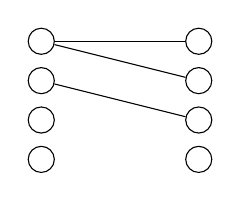
\begin{tikzpicture}[scale=1, auto=center]
\tikzstyle{every node}=[draw,shape=circle];
  \node[minimum size=0.25cm] (n1) at (0,1.5) {};
  \node[minimum size=0.25cm] (n2) at (0,1) {};
  \node[minimum size=0.25cm] (n3) at (0,0.5) {};
  \node[minimum size=0.25cm] (n4) at (0,0) {};
  \node[minimum size=0.25cm] (n5) at (2,1.5) {};
  \node[minimum size=0.25cm] (n6) at (2,1) {};
  \node[minimum size=0.25cm] (n7) at (2,0.5) {};
  \node[minimum size=0.25cm] (n8) at (2,0) {};

  \foreach \from/\to in {n1/n5,n1/n6,n2/n7}
    \draw (\from) -- (\to);
\end{tikzpicture}
\end{subfigure}
\begin{subfigure}{0.24\textwidth}
\centering
\caption{$H_{15-16}$: $4 / 8$}
\label{Fig2_8}

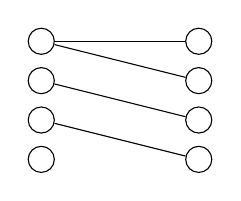
\begin{tikzpicture}[scale=1, auto=center]
\tikzstyle{every node}=[draw,shape=circle];
  \node[minimum size=0.25cm] (n1) at (0,1.5) {};
  \node[minimum size=0.25cm] (n2) at (0,1) {};
  \node[minimum size=0.25cm] (n3) at (0,0.5) {};
  \node[minimum size=0.25cm] (n4) at (0,0) {};
  \node[minimum size=0.25cm] (n5) at (2,1.5) {};
  \node[minimum size=0.25cm] (n6) at (2,1) {};
  \node[minimum size=0.25cm] (n7) at (2,0.5) {};
  \node[minimum size=0.25cm] (n8) at (2,0) {};

  \foreach \from/\to in {n1/n5,n1/n6,n2/n7,n3/n8}
    \draw (\from) -- (\to);
\end{tikzpicture}
\end{subfigure}

%\vspace{0.25cm}
\begin{subfigure}{0.24\textwidth}
\centering
\caption{$H_{17}$: $4 / 8$}
\label{Fig2_9}

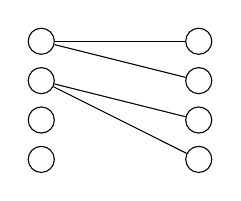
\begin{tikzpicture}[scale=1, auto=center]
\tikzstyle{every node}=[draw,shape=circle];
  \node[minimum size=0.25cm] (n1) at (0,1.5) {};
  \node[minimum size=0.25cm] (n2) at (0,1) {};
  \node[minimum size=0.25cm] (n3) at (0,0.5) {};
  \node[minimum size=0.25cm] (n4) at (0,0) {};
  \node[minimum size=0.25cm] (n5) at (2,1.5) {};
  \node[minimum size=0.25cm] (n6) at (2,1) {};
  \node[minimum size=0.25cm] (n7) at (2,0.5) {};
  \node[minimum size=0.25cm] (n8) at (2,0) {};

  \foreach \from/\to in {n1/n5,n1/n6,n2/n7,n2/n8}
    \draw (\from) -- (\to);
\end{tikzpicture}
\end{subfigure}
\begin{subfigure}{0.24\textwidth}
\centering
\caption{$H_{18-20}$: $4 / 8$}
\label{Fig2_10}

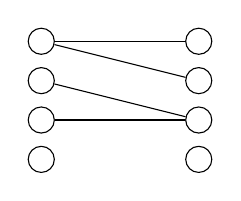
\begin{tikzpicture}[scale=1, auto=center]
\tikzstyle{every node}=[draw,shape=circle];
  \node[minimum size=0.25cm] (n1) at (0,1.5) {};
  \node[minimum size=0.25cm] (n2) at (0,1) {};
  \node[minimum size=0.25cm] (n3) at (0,0.5) {};
  \node[minimum size=0.25cm] (n4) at (0,0) {};
  \node[minimum size=0.25cm] (n5) at (2,1.5) {};
  \node[minimum size=0.25cm] (n6) at (2,1) {};
  \node[minimum size=0.25cm] (n7) at (2,0.5) {};
  \node[minimum size=0.25cm] (n8) at (2,0) {};

  \foreach \from/\to in {n1/n5,n1/n6,n2/n7,n3/n7}
    \draw (\from) -- (\to);
\end{tikzpicture}
\end{subfigure}
\begin{subfigure}{0.24\textwidth}
\centering
\caption{$H_{21-22}$: $5 / 6$}
\label{Fig2_11}

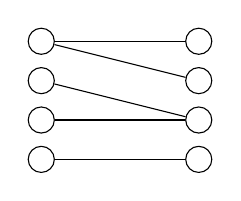
\begin{tikzpicture}[scale=1, auto=center]
\tikzstyle{every node}=[draw,shape=circle];
  \node[minimum size=0.25cm] (n1) at (0,1.5) {};
  \node[minimum size=0.25cm] (n2) at (0,1) {};
  \node[minimum size=0.25cm] (n3) at (0,0.5) {};
  \node[minimum size=0.25cm] (n4) at (0,0) {};
  \node[minimum size=0.25cm] (n5) at (2,1.5) {};
  \node[minimum size=0.25cm] (n6) at (2,1) {};
  \node[minimum size=0.25cm] (n7) at (2,0.5) {};
  \node[minimum size=0.25cm] (n8) at (2,0) {};

  \foreach \from/\to in {n1/n5,n1/n6,n2/n7,n3/n7,n4/n8}
    \draw (\from) -- (\to);
\end{tikzpicture}
\end{subfigure}
\begin{subfigure}{0.24\textwidth}
\centering
\caption{$H_{23}$: $4 / 4$}
\label{Fig2_12}

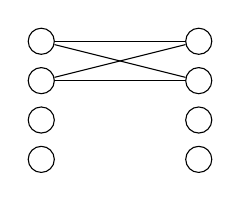
\begin{tikzpicture}[scale=1, auto=center]
\tikzstyle{every node}=[draw,shape=circle];
  \node[minimum size=0.25cm] (n1) at (0,1.5) {};
  \node[minimum size=0.25cm] (n2) at (0,1) {};
  \node[minimum size=0.25cm] (n3) at (0,0.5) {};
  \node[minimum size=0.25cm] (n4) at (0,0) {};
  \node[minimum size=0.25cm] (n5) at (2,1.5) {};
  \node[minimum size=0.25cm] (n6) at (2,1) {};
  \node[minimum size=0.25cm] (n7) at (2,0.5) {};
  \node[minimum size=0.25cm] (n8) at (2,0) {};

  \foreach \from/\to in {n1/n5,n1/n6,n2/n5,n2/n6}
    \draw (\from) -- (\to);
\end{tikzpicture}
\end{subfigure}

%\vspace{0.25cm}
\begin{subfigure}{0.24\textwidth}
\centering
\caption{$H_{24}$: $5 / 4$}
\label{Fig2_13}

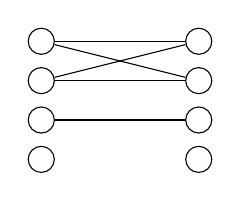
\begin{tikzpicture}[scale=1, auto=center]
\tikzstyle{every node}=[draw,shape=circle];
  \node[minimum size=0.25cm] (n1) at (0,1.5) {};
  \node[minimum size=0.25cm] (n2) at (0,1) {};
  \node[minimum size=0.25cm] (n3) at (0,0.5) {};
  \node[minimum size=0.25cm] (n4) at (0,0) {};
  \node[minimum size=0.25cm] (n5) at (2,1.5) {};
  \node[minimum size=0.25cm] (n6) at (2,1) {};
  \node[minimum size=0.25cm] (n7) at (2,0.5) {};
  \node[minimum size=0.25cm] (n8) at (2,0) {};

  \foreach \from/\to in {n1/n5,n1/n6,n2/n5,n2/n6,n3/n7}
    \draw (\from) -- (\to);
\end{tikzpicture}
\end{subfigure}
\begin{subfigure}{0.24\textwidth}
\centering
\caption{$H_{25}$: $6 / 4$}
\label{Fig2_14}

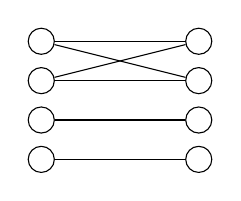
\begin{tikzpicture}[scale=1, auto=center]
\tikzstyle{every node}=[draw,shape=circle];
  \node[minimum size=0.25cm] (n1) at (0,1.5) {};
  \node[minimum size=0.25cm] (n2) at (0,1) {};
  \node[minimum size=0.25cm] (n3) at (0,0.5) {};
  \node[minimum size=0.25cm] (n4) at (0,0) {};
  \node[minimum size=0.25cm] (n5) at (2,1.5) {};
  \node[minimum size=0.25cm] (n6) at (2,1) {};
  \node[minimum size=0.25cm] (n7) at (2,0.5) {};
  \node[minimum size=0.25cm] (n8) at (2,0) {};

  \foreach \from/\to in {n1/n5,n1/n6,n2/n5,n2/n6,n3/n7,n4/n8}
    \draw (\from) -- (\to);
\end{tikzpicture}
\end{subfigure}
\begin{subfigure}{0.24\textwidth}
\centering
\caption{$H_{26}$: $6 / 4$}
\label{Fig2_15}

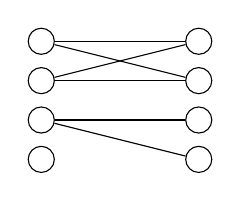
\begin{tikzpicture}[scale=1, auto=center]
\tikzstyle{every node}=[draw,shape=circle];
  \node[minimum size=0.25cm] (n1) at (0,1.5) {};
  \node[minimum size=0.25cm] (n2) at (0,1) {};
  \node[minimum size=0.25cm] (n3) at (0,0.5) {};
  \node[minimum size=0.25cm] (n4) at (0,0) {};
  \node[minimum size=0.25cm] (n5) at (2,1.5) {};
  \node[minimum size=0.25cm] (n6) at (2,1) {};
  \node[minimum size=0.25cm] (n7) at (2,0.5) {};
  \node[minimum size=0.25cm] (n8) at (2,0) {};

  \foreach \from/\to in {n1/n5,n1/n6,n2/n5,n2/n6,n3/n7,n3/n8}
    \draw (\from) -- (\to);
\end{tikzpicture}
\end{subfigure}
\begin{subfigure}{0.24\textwidth}
\centering
\caption{$H_{27}$: $8 / 4$}
\label{Fig2_16}

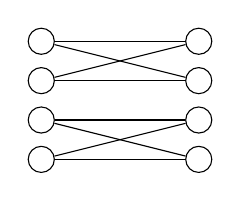
\begin{tikzpicture}[scale=1, auto=center]
\tikzstyle{every node}=[draw,shape=circle];
  \node[minimum size=0.25cm] (n1) at (0,1.5) {};
  \node[minimum size=0.25cm] (n2) at (0,1) {};
  \node[minimum size=0.25cm] (n3) at (0,0.5) {};
  \node[minimum size=0.25cm] (n4) at (0,0) {};
  \node[minimum size=0.25cm] (n5) at (2,1.5) {};
  \node[minimum size=0.25cm] (n6) at (2,1) {};
  \node[minimum size=0.25cm] (n7) at (2,0.5) {};
  \node[minimum size=0.25cm] (n8) at (2,0) {};

  \foreach \from/\to in {n1/n5,n2/n6,n3/n7,n4/n8}
    \draw[dashed] (\from) -- (\to);
  \foreach \from/\to in {n1/n5,n1/n6,n2/n5,n2/n6,n3/n7,n3/n8,n4/n7,n4/n8}
    \draw (\from) -- (\to);
\end{tikzpicture}
\end{subfigure}

%\vspace{0.25cm}
\begin{subfigure}{0.24\textwidth}
\centering
\caption{$H_{28}$: $3 / 6$}
\label{Fig2_17}

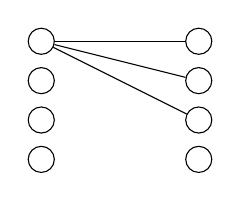
\begin{tikzpicture}[scale=1, auto=center]
\tikzstyle{every node}=[draw,shape=circle];
  \node[minimum size=0.25cm] (n1) at (0,1.5) {};
  \node[minimum size=0.25cm] (n2) at (0,1) {};
  \node[minimum size=0.25cm] (n3) at (0,0.5) {};
  \node[minimum size=0.25cm] (n4) at (0,0) {};
  \node[minimum size=0.25cm] (n5) at (2,1.5) {};
  \node[minimum size=0.25cm] (n6) at (2,1) {};
  \node[minimum size=0.25cm] (n7) at (2,0.5) {};
  \node[minimum size=0.25cm] (n8) at (2,0) {};

  \foreach \from/\to in {n1/n5,n1/n6,n1/n7}
    \draw (\from) -- (\to);
\end{tikzpicture}
\end{subfigure}
\begin{subfigure}{0.24\textwidth}
\centering
\caption{$H_{29}$: $4 / 6$}
\label{Fig2_18}

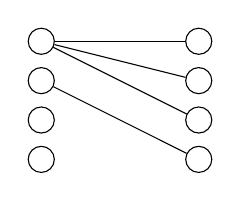
\begin{tikzpicture}[scale=1, auto=center]
\tikzstyle{every node}=[draw,shape=circle];
  \node[minimum size=0.25cm] (n1) at (0,1.5) {};
  \node[minimum size=0.25cm] (n2) at (0,1) {};
  \node[minimum size=0.25cm] (n3) at (0,0.5) {};
  \node[minimum size=0.25cm] (n4) at (0,0) {};
  \node[minimum size=0.25cm] (n5) at (2,1.5) {};
  \node[minimum size=0.25cm] (n6) at (2,1) {};
  \node[minimum size=0.25cm] (n7) at (2,0.5) {};
  \node[minimum size=0.25cm] (n8) at (2,0) {};

  \foreach \from/\to in {n1/n5,n1/n6,n1/n7,n2/n8}
    \draw (\from) -- (\to);
\end{tikzpicture}
\end{subfigure}
\begin{subfigure}{0.24\textwidth}
\centering
\caption{$H_{30}$: $5 / 6$}
\label{Fig2_19}

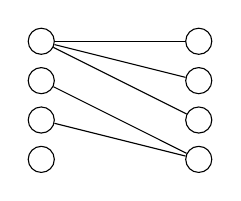
\begin{tikzpicture}[scale=1, auto=center]
\tikzstyle{every node}=[draw,shape=circle];
  \node[minimum size=0.25cm] (n1) at (0,1.5) {};
  \node[minimum size=0.25cm] (n2) at (0,1) {};
  \node[minimum size=0.25cm] (n3) at (0,0.5) {};
  \node[minimum size=0.25cm] (n4) at (0,0) {};
  \node[minimum size=0.25cm] (n5) at (2,1.5) {};
  \node[minimum size=0.25cm] (n6) at (2,1) {};
  \node[minimum size=0.25cm] (n7) at (2,0.5) {};
  \node[minimum size=0.25cm] (n8) at (2,0) {};

  \foreach \from/\to in {n1/n5,n1/n6,n1/n7,n2/n8,n3/n8}
    \draw (\from) -- (\to);
\end{tikzpicture}
\end{subfigure}
\begin{subfigure}{0.24\textwidth}
\centering
\caption{$H_{31}$: $6 / 6$}
\label{Fig2_20}

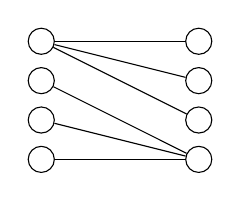
\begin{tikzpicture}[scale=1, auto=center]
\tikzstyle{every node}=[draw,shape=circle];
  \node[minimum size=0.25cm] (n1) at (0,1.5) {};
  \node[minimum size=0.25cm] (n2) at (0,1) {};
  \node[minimum size=0.25cm] (n3) at (0,0.5) {};
  \node[minimum size=0.25cm] (n4) at (0,0) {};
  \node[minimum size=0.25cm] (n5) at (2,1.5) {};
  \node[minimum size=0.25cm] (n6) at (2,1) {};
  \node[minimum size=0.25cm] (n7) at (2,0.5) {};
  \node[minimum size=0.25cm] (n8) at (2,0) {};

  \foreach \from/\to in {n1/n5,n1/n6,n1/n7,n2/n8,n3/n8,n4/n8}
    \draw (\from) -- (\to);
\end{tikzpicture}
\end{subfigure}

\captionsetup{justification=centerfirst}
\caption{Balanced bipartite graphs with eight nodes and type constraints \\ \vspace{0.2cm}
\footnotesize{\emph{Notes}: Solid lines indicate the type constraints. \\
%Group winners are the nodes on the left-hand side, runners-up are the nodes on the right-hand side. \\
The first (second) number shows the number of type exclusions (the number of valid assignments).}}
\label{Fig2}
\end{figure}

%\end{document}